\documentclass{standalone}
\usepackage{tikz}
\usetikzlibrary{arrows.meta}

\begin{document}
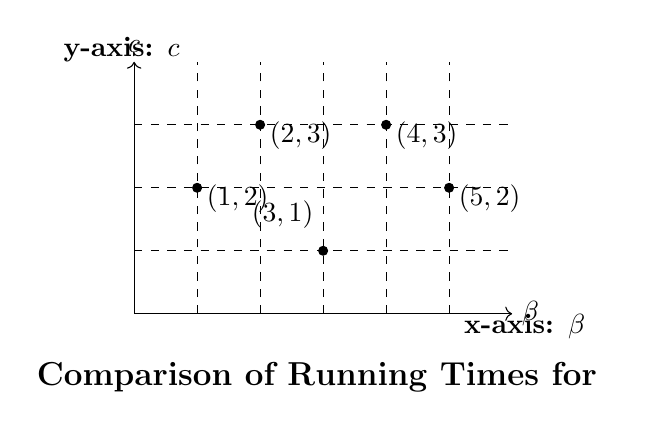
\begin{tikzpicture}[scale=0.8]
    % Axis setup
    \draw[->] (0,0) -- (6,0) node[right] {$\beta$};
    \draw[->] (0,0) -- (0,4) node[above] {$c$};

    % Grid lines
    \foreach \x in {1,...,5} \draw[dashed] (\x,0) -- (\x,4);
    \foreach \y in {1,...,3} \draw[dashed] (0,\y) -- (6,\y);

    % Dots representing data points
    \filldraw (1,2) circle[radius=2pt];
    \filldraw (2,3) circle[radius=2pt];
    \filldraw (3,1) circle[radius=2pt];
    \filldraw (4,3) circle[radius=2pt];
    \filldraw (5,2) circle[radius=2pt];

    % Labels for dots
    \node at (1,2.2) [below right] {$(1, 2)$};
    \node at (2,3.2) [below right] {$(2, 3)$};
    \node at (3,1.2) [above left] {$(3, 1)$};
    \node at (4,3.2) [below right] {$(4, 3)$};
    \node at (5,2.2) [below right] {$(5, 2)$};

    % Axes labels
    \node at (6.2,-0.2) {$\textbf{x-axis: } \beta$};
    \node at (-0.2,4.2) {$\textbf{y-axis: } c$};

    % Title
    \node at (3,-1) [font=\large\bfseries] {Comparison of Running Times for $\fvs$};
\end{tikzpicture}
\end{document}